\documentclass{article}
\usepackage[utf8]{inputenc}
\setlength\parindent{0pt}
\usepackage{amsmath}
\usepackage{amsfonts}
\usepackage{amssymb}
\usepackage{comment}
\usepackage{natbib}
\usepackage{graphicx}
\usepackage{float}
\usepackage{mathtools}
\usepackage{caption}
\usepackage{subcaption}
\usepackage{geometry}
\usepackage{bm}
\usepackage{hyperref}
\usepackage{emoji}
 \geometry{
 a4paper,
 total={170mm,257mm},
 left=30mm,
 right=30mm,
 top=30mm,
 bottom=30mm
}

\setlength{\parskip}{\baselineskip}

\title{A Brief Introduction to Likelihood Theory}
\date{}
\begin{document}
\maketitle

We take basic statistical estimators for granted. For example, for a distribution with mean $\mu$, we estimate it using $\overline{\mathbf{x}}:=\sum_i x_i/n$. But why exactly \textit{that} equation? This is a small supplement if you'd like a really good answer to that.

\section{Probability and Likelihood}

We tend to talk about probability, $\mathbb{P}(\mathbf{X}|\boldsymbol{\theta})$, for data $\mathbf{X}$ and parameters $\boldsymbol{\theta}$\footnote{Going forward I'm going to bold things that are either vectors or matrices, and otherwise everything else is a single number.}. For example, $\mathbf{X}$ could be an array of numbers and $\boldsymbol{\theta}$ might be mean and standard deviation, $\{\mu, \sigma\}$. The basic way to estimate $\boldsymbol{\theta}$ would be to look at a related function, the \textit{likelihood}, which is the probability of the parameters given the data: $\mathcal{L}(\boldsymbol{\theta}|\mathbf{X}) \propto \mathbb{P}(\boldsymbol{\theta}|\mathbf{X})$ (more on this in a bit). After all, this is the situation we find ourselves in in real life: given that I have this data $\mathbf{X}$, what are the most likely guesses of the statistics I'm interested in $\boldsymbol{\theta}$? We will simply take the maximum of this function. This is called...
\begin{center}
\emoji{sparkles}\textbf{\textit{Maximum Likelihood Estimation}}\emoji{sparkles}
\end{center}

If the likelihood is smooth and convex (like a dirt mound or something), then the maximum corresponds to the unique point where there is no slope. Furthermore, we can get a sense of how "maximumy" that point is by looking at the best-fitting parabola centered at the best guess for the maximum. The technical terms for these is the \textit{score} and the \textit{information}, respectively, and will be calculated by taking the first and second derivatives of the likelihood. Here's a general picture of what we're looking to find, and the other things we'll calculate for a single parameter:

\begin{figure}[H]
    \centering
    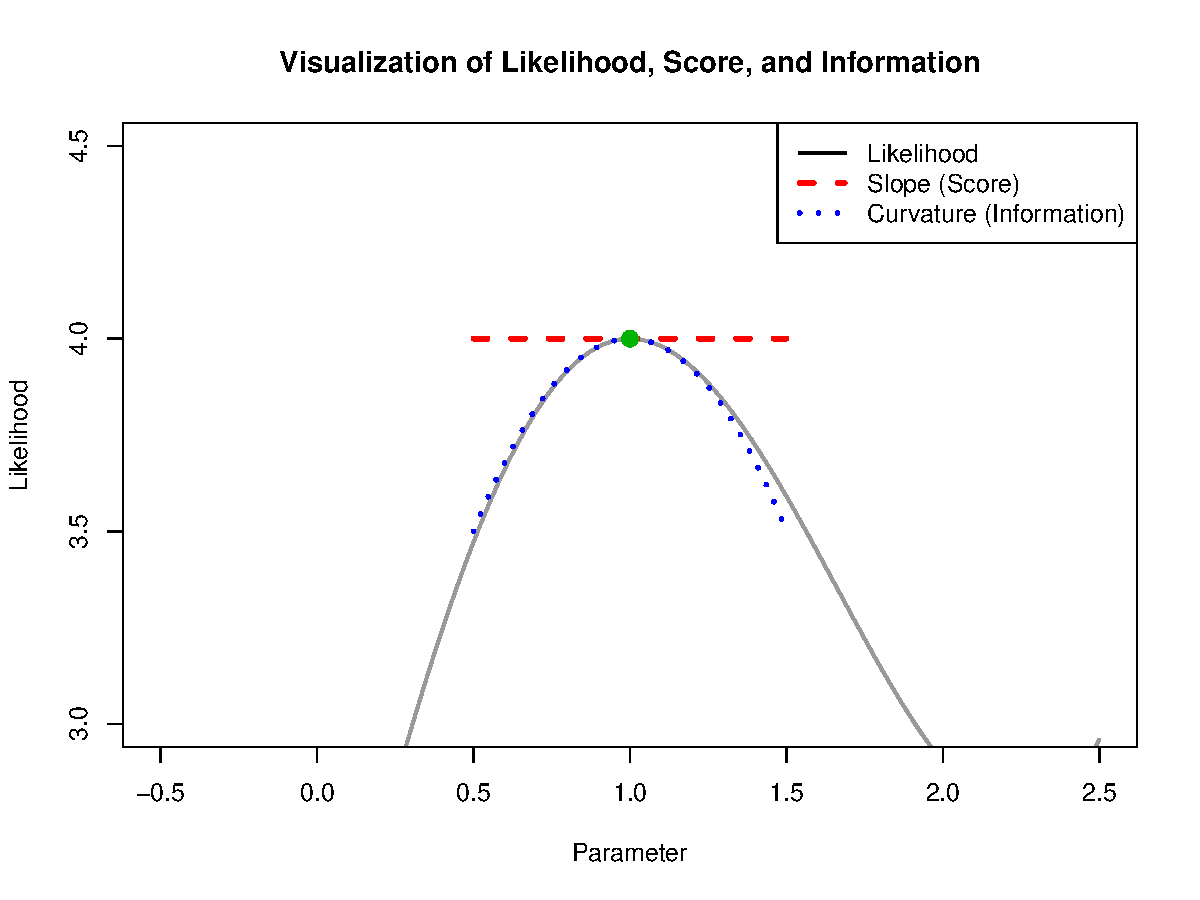
\includegraphics[width=0.8\textwidth]{likelihood_plot.pdf}
    \label{fig:likelihood_plot}
    \caption{Conceptual visualization of likelihood, score, and information}
\end{figure}

Keep in mind that while this function is smooth as we vary $\theta$, the data it's defined on is random, making our maximum point only an estimate of the truth. Also, the curvature of the parabola is directly related to the variance of the estimate itself: in fact, it's the inverse! Let me say that again: the \textit{variance} of our estimator is the inverse of the \textit{information} we have about it. This is a rare case where statisticians have given crisp, meaningful names to important concepts.

\subsection{How probability and likelihood are related}
This subsection is designed to be crystal clear about what likelihood is, and why it's conceptually different from probability. The subtle difference between them is the reversal of what is conditional:

\begin{itemize}
    \item Probability: $\mathbb{P}(\mathbf{X}|\boldsymbol{\theta})$ - the probability of observing data $\mathbf{X}$ given parameters $\boldsymbol{\theta}$.
    \item Likelihood: $\mathbb{P}(\boldsymbol{\theta}|\mathbf{X})$ - how likely the parameters $\boldsymbol{\theta}$ are, given the observed data $\mathbf{X}$.
\end{itemize}

I want to motivate this distinction more mathematically, and let's start from basic principles about what conditional probability is. For any two things that might happen $A$ and $B$ (and the event of both happening is $A\cap B$), the definition of a conditional probability is\footnote{Note that this only makes sense if $\mathbb{P}(B)>0$. The math required to make sense of conditionals in the general case is an eldritch horror which is best kept in its accursed crypt.}:

\begin{equation}
\mathbb{P}(A|B) := \frac{\mathbb{P}(A \cap B)}{\mathbb{P}(B)}
\end{equation}

\newpage
This means that assuming $B$ happens, what's the probability that $A$ happens in addition to $B$. We will certainly get more intuition about conditional probability later in class. Rearranging the above equation, $\mathbb{P}(A|B)\cdot\mathbb{P}(B) = \mathbb{P}(A \cap B)$. Also, $A$ and $B$ could be anything, so you could also write $\mathbb{P}(B|A)\mathbb{P}(A) = \mathbb{P}(B \cap A)$. Finally, because $\mathbb{P}(A \cap B)=\mathbb{P}(B \cap A)$ (it's symmetric), then it follows:

\begin{equation}
\mathbb{P}(A|B)\mathbb{P}(B) = \mathbb{P}(B|A)\mathbb{P}(A)
\end{equation}

Rearranging slightly, we get:

\begin{equation}
\mathbb{P}(A|B) = \frac{\mathbb{P}(B|A)\mathbb{P}(A)}{\mathbb{P}(B)}
\end{equation}

This happens to be called \textit{Bayes' Theorem}, and we'll talk more about it later in class soon. For now, it's barely a profound theorem at all, just a straightforward rewriting of some basic probability concepts. Getting back to likelihood, let's apply this to our context of data $\textbf{X}$ and parameters $\boldsymbol{\theta}$:

\begin{equation}
\mathbb{P}(\boldsymbol{\theta}|\textbf{X}) = \frac{\mathbb{P}(\textbf{X}|\boldsymbol{\theta})\mathbb{P}(\boldsymbol{\theta})}{\mathbb{P}(\textbf{X})}
\end{equation}

In traditional (\textit{frequentist}) likelihood theory, we often ignore $\mathbb{P}(\boldsymbol{\theta})$, as if to say as don't have a guess about the parameters' values absent any data.\footnote{A \textit{bayesian} (as they call themselves) would definitely NOT ignore this, and criticize this whole approach for doing so. This is a deep philosophical tension tbh.} Also, $\mathbb{P}(\mathbf{X})$ is just a constant with respect to $\boldsymbol{\theta}$, so maximizing the likelihood doesn't depend on that at all. So as long as we're happy ignoring $\mathbb{P}(\boldsymbol{\theta})$ we have:

\begin{equation}
\mathcal{L}(\boldsymbol{\theta}|\mathbf{X}) := \mathbb{P}(\boldsymbol{\theta}|\mathbf{X}) \propto \mathbb{P}(\mathbf{X}|\boldsymbol{\theta})
\end{equation}

So importantly, when switching our thinking to likelihood, we actually just use the equations associated with the probability itself. Nothing about the forms of the distributions involved change, we just shift our attention to maximizing the parameters $\boldsymbol{\theta}$.

Last comment, if the observations $\mathbf{X} = \{X_1, X_2, ..., X_n\}$ are independent, the likelihood is proportional to the \textit{product} of individual probabilities:

\begin{equation}
\mathcal{L}(\boldsymbol{\theta}|X_1, X_2, ..., X_n) \propto \mathbb{P}(X_1, X_2, ..., X_n)|\boldsymbol{\theta}) = \prod_{i=1}^n \mathbb{P}(X_i|\boldsymbol{\theta})
\end{equation}

\section{Maximizing Likelihood}

Now that we've pinned down what likelihood is, let's maximize it with respect to our statistics of choice $\boldsymbol{\theta}$. For a smooth likelihood function, the maximum occurs where the derivative is zero in all directions. Mathematically:

\begin{equation}
\frac{\partial \mathcal{L}(\boldsymbol{\theta}|\mathbf{X})}{\partial \boldsymbol{\theta}} = \mathbf{0}
\end{equation}

Solving this equation to be equal to zero is where the rubber meets the road. That is, it's how we \textit{derive} the estimates we use. Consider that it's easier to maximize the log of the likelihood, which will also maximize the actual likelihood, as it's a monotone increasing function. We do that because it's more convenient, as it transforms products into sums:

\begin{equation}
\ell(\boldsymbol{\theta}|\mathbf{X}) := \log \mathcal{L}(\boldsymbol{\theta}|\mathbf{X})
\end{equation}

The \textit{score} is defined as the partial derivative of the log-likelihood function with respect to its parameters:

\begin{equation}
\mathcal{S}(\boldsymbol{\theta}) := \frac{\partial \ell(\boldsymbol{\theta}|\mathbf{X})}{\partial \mathbf{\theta}}
\end{equation}

This is the thing we will solve to be zero, and doing so will give us our maximum likelihood estimates $\hat{\boldsymbol{\theta}}$.

\section{Information and Variance}

The (Fisher)\footnote{Named after R.A. Fisher, a foundationally important statistical theorist.} \textit{information} is a measure of the amount of information that data $\mathbf{X}$ carries about an unknown parameters
$\boldsymbol{\theta}$. It's defined as the negative expected value of the \textit{second} derivative of the log-likelihood function:

\begin{equation}
\mathcal{I}(\boldsymbol{\theta}) = -\mathbb{E}\left[\frac{\partial^2 \ell(\boldsymbol{\theta}|\mathbf{X})}{\partial \boldsymbol{\theta}^2}\right]
\end{equation}

(Don't worry about the expected value part ``$\mathbb{E}$'' if it's not familiar, the ideas and examples in this doc it won't change at all, I just want to be precise.) Conceptually, this corresponds to the level of curvature in the parabola in Figure 1. Information is the inverse of the variance of the estimator:

\begin{equation}
Var(\hat{\boldsymbol{\theta}}) = \mathcal{I}(\boldsymbol{\theta})^{-1}
\end{equation}

The mathematical reasons are a bit too deep to go into here, but it does make intuitive sense: the more information about an estimator you have, the less variance it will exhibit if you repeatedly got a fresh dataset and calculated the maximum-likelihood estimate.

\section{Example 1: Normal Distribution}

Alright, let's make these concepts thumpingly concrete by demonstrating them. Let's start with a univariate normal distribution. Suppose we have a sample $\mathbf{X}=\{X_1, ..., X_n\}$ drawn from a normal distribution with unknown mean $\mu$ and known variance $\sigma^2$, and we want an estimate of the mean $\hat{\mu}$. We know this should be the average $\sum_i x_i / n$, but we'll derive it and watch it appear before our very eyes! \emoji{eyes}

The \href{https://en.wikipedia.org/wiki/Normal_distribution}{likelihood function} is:

\begin{equation}
\mathcal{L}(\mu|\mathbf{X}) = \prod_{i=1}^n \frac{1}{\sqrt{2\pi\sigma^2}} \exp\left(-\frac{(X_i - \mu)^2}{2\sigma^2}\right)
\end{equation}

The log-likelihood is:

\begin{equation}
\ell(\mu|\mathbf{X}) = -\frac{n}{2}\log(2\pi\sigma^2) - \frac{1}{2\sigma^2}\sum_{i=1}^n (X_i - \mu)^2
\end{equation}

So the score is:

\begin{equation}
\mathcal{S}(\mu) = \frac{\partial \ell(\mu|\boldsymbol{X})}{\partial \mu} = \frac{1}{\sigma^2}\sum_{i=1}^n (X_i - \mu)
\end{equation}

Setting this to zero and solving gives us the MLE for $\mu$:

\begin{equation}
\hat{\mu} = \frac{1}{n}\sum_{i=1}^n X_i
\end{equation}

To find the information, we take the negative expectation of the second derivative of the log-likelihood:

\begin{equation}
\mathcal{I}(\mu) = -\mathbb{E}\left[\frac{\partial^2 \ell(\mu|\mathbf{X})}{\partial \mu^2}\right] = \frac{n}{\sigma^2}
\end{equation}

So the variance of the estimator is $\mathcal{I}(\mu)^{-1} = \sigma^2/n$. It's not a coincidence that this matches the guarantees of the Central Limit Theorem! The variance of an average is the variance of the original population, divided by the sample size.

\section{Example 2: Multivariate Linear Regression}

We're getting slightly ahead of ourselves, but let's do a more athletic example, multivariate linear regression. If you don't follow all of the derivation in this example it's not a problem at all, but if you did decide to brush up on your linear algebra and calculus, you should be able to follow it. Here's the model in this case:

\begin{equation}
\mathbf{y} = \mathbf{X}\bm{\beta} + \bm{\epsilon}
\end{equation}

Where:
\begin{itemize}
    \item $\mathbf{y}$ is the outcome (an $n \times 1$ vector)
    \item $\mathbf{X}$ is our data (an $n \times p$ matrix of predictors)
    \item $\bm{\beta}$ is our fitted coefficients (a $p \times 1$ vector)
    \item $\bm{\epsilon}$ are the errors (an $n \times 1$ vector)
\end{itemize}

If the errors are independent (the scope of this course) and normally distributed (an assumption of linear regression anyways), the likelihood function is:

\begin{equation}
\mathcal{L}(\bm{\beta}, \sigma^2|\mathbf{y},\mathbf{X}) = (2\pi\sigma^2)^{-n/2} \exp\left(-\frac{1}{2\sigma^2}(\mathbf{y} - \mathbf{X}\bm{\beta})^T(\mathbf{y} - \mathbf{X}\bm{\beta})\right)
\end{equation}

Maximizing this directly would be horrible, but as typical it's better after taking the log:

\begin{equation}
\ell(\bm{\beta}, \sigma^2|\mathbf{y},\mathbf{X}) = -\frac{n}{2}\log(2\pi\sigma^2) - \frac{1}{2\sigma^2}(\mathbf{y} - \mathbf{X}\bm{\beta})^T(\mathbf{y} - \mathbf{X}\bm{\beta})
\end{equation}

To find the maximum likelihood estimate of $\bm{\beta}$, we differentiate the log-likelihood with respect to $\bm{\beta}$ (the score)\footnote{This differentiation might seem to come from nowhere, but this is using the logic of \href{https://www2.imm.dtu.dk/pubdb/pubs/3274-full.html}{differentiation for matrices}, and is good to keep fresh.}:

\begin{equation}
\mathcal{S}(\boldsymbol{\beta}) = \frac{\partial \ell}{\partial \bm{\beta}} = \frac{1}{\sigma^2}\mathbf{X}^T(\mathbf{y} - \mathbf{X}\bm{\beta})
\end{equation}

Setting this to zero and solving for $\bm{\beta}$:

\begin{equation}
\mathbf{X}^T\mathbf{X}\bm{\beta} = \mathbf{X}^T\mathbf{y}
\end{equation}

\begin{equation}
\Rightarrow \boxed{\hat{\bm{\beta}} = (\mathbf{X}^T\mathbf{X})^{-1}\mathbf{X}^T\mathbf{y}}
\end{equation}

This is the closed-form solution for the maximum likelihood estimates in multivariate linear regression! You can see that all it takes to compute them in practice is to do a matrix multiplication, take an inverse, then two more matrix multiplications. Deceptively simple at the end of it all. Let's go on and derive the information, taking the negative expectated value of the second derivative of the log-likelihood with respect to $\bm{\beta}$:

\begin{equation}
\mathcal{I}(\bm{\beta}) = -\mathbb{E}\left[\frac{\partial^2 \ell}{\partial \bm{\beta} \ \partial\bm{\beta}^T}\right] = \frac{1}{\sigma^2}\mathbf{X}^T\mathbf{X}
\end{equation}

Taking the inverse, the covariance matrix is:

\begin{equation}
Var(\hat{\bm{\beta}}) = \sigma^2(\mathbf{X}^T\mathbf{X})^{-1}
\end{equation}

You can then use these to form confidence intervals, do hypothesis testing, whatever you'd like. That's it! That's literally everything you need to know to do maximum likelihood estimation yourself!

\end{document}